\documentclass[paper=a4, parskip=half-]{scrartcl}
\usepackage[utf8]{inputenc}

\usepackage{amsmath}
\usepackage{mathtools}
\usepackage{marvosym} % for the \Lightning symbol
\usepackage{amssymb} % more icons/symbols
\usepackage{tablefootnote} % for footnotes in tables
% not in standard texlive, can't be asked to figure it out now
%\usepackage{ccicons} % creative commons icon
\usepackage{hyperref} % for hyper links
\usepackage[dvipsnames]{xcolor} % to color stuff -- dvipnames for additional color names
\usepackage[shortlabels]{enumitem} % to modify enumeration labels
\usepackage{tcolorbox} % for colored boxes - see https://tex.stackexchange.com/questions/66154/how-to-construct-a-coloured-box-with-rounded-corners/172608#172608
\usepackage{tikz} % drawing stuff
\usepackage{eurosym} % € (no, default LaTeX font doesn't include it)
\usepackage{natbib}
\usepackage{graphicx}

\usepackage{listings}

\usepackage{geometry}
 \geometry{
 a4paper,
 left=20mm,
 right=20mm,
 top=20mm,
 bottom=30mm,
 }


\title{Advanced Topics of Communication Systems}
\author{\texttt{\{wnicole\}@ethz.ch}}
\date{ETH Zürich, HS 2020}

% Custom commands
\newcommand{\setzeroone}{\lbrace 0, 1 \rbrace} % => {0,1} (Notice the missing $$)
\newcommand{\horizontaldivider}{\begin{center} \line(1,0){350} \end{center}}

\begin{document}

\begin{titlepage}
\maketitle
\vspace{5cm}
\thispagestyle{empty}


\begin{abstract}
This is a summary for the course \textit{Advanced Topics of Communication Systems} at ETH Zürich.

I do not guarantee correctness or completeness, nor is this document endorsed by the lecturers.
Feel free to point out any erratas. This summary was written in a very short time frame and might not be the most structured.
\end{abstract}

\end{titlepage}

\tableofcontents
%\listoffigures
%\listoftables
\newpage

\section{Traffic Engineering}

\subsection{Label Switching}

\paragraph{Packet vs. Circuit Switching}
In packet switching, source sends information as self-contained packets with an address and each packet travels independently to the destination (stateless forwarding at routers) - the destination then recreates the message. In circuit switching, the source first establishes a connection to the destination (reserved bandwidth) and data goes over this reserved path - the connection needs to be established and torn down.

CS guarantees bandwidth and predictable performance, switch design is very simple, adding QoS measures is easy - but, inefficient (esp. for bursty traffic) and overhead.

\paragraph{Virtual Circuits}
Basis of traffic engineering. Forwarding based on a virtual circuit identifier that identify long-lived streams of data that can be scheduled. Each link carries many virtual circuits. Can support various QoS measures (guarantees).

Still does storing and forwarding and still needs buffers. Multiplexing on a link is similar to time sharing (with or without reservations).

\paragraph{Multiprotocol Label Switching (MPLS)}
A layer 2.5 protocol (Ethernet, MPLS header stack, IP) implementing unidirectional virtual circuits = label switched path (LSP) in an IP network. Allows for implementation of TE, QoS, fast reroute, VPNs and more.

A label-switching router inspects an inbound packet's label and input port (per-interface / per-device basis) and according to its forwarding table (single look-up) then decides the output port and next packet label (next hop). At the edge of an MPLS network, labels are either pushed or popped on/off the MPLS label header stack and at the core the top-most label is swapped.

\begin{figure}[h]
	\centering
	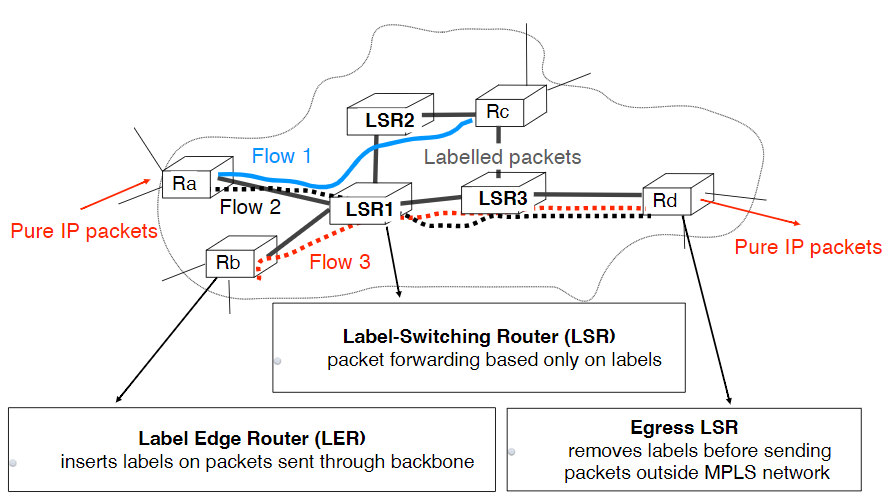
\includegraphics[scale=0.6]{images/1-mpls.PNG}
	\caption{Integrating label swapping and IP.}
	\label{fig:mpls}
\end{figure}

%TODO: more outsourced MPLS info, header etc. also whys
%TODO: lec 4 MPLS in practice (end)?

\paragraph{Forwarding Equivalence Class (FEC)}
Group of IP packets that are forwarded in the same manner. FECs can be used to associate the same label to all packets that belong to the same FEC (usually pushed by a LER). Typically destination IP address, sometimes QoS class.

\paragraph{Distributing Labels}
There are various ways to fill the forwarding tables of all LSRs in a given network. Dedicated protocols, such as LDP and RSVP-TE, can be used to distribute FEC-label mappings. Or mappings can be put inside messages sent by existing routing protocols (that are extensible, such as BGP).

FEC-label mappings are determined by the downstream LSR (destination), which sends them to the upstream one (source). This is either done on demand (space-friendly, not very failure resistant since no backup specified) or in an unsolicited / independent manner (failure resistant by knowing all possibilities, timing is hard).

\paragraph{Label Distribution Protocol (LDP)}
LDP relies on the underlying routing information provided by an IGP (e.g. OSPF, BGP, etc.) in order to forward label packets. Hop-by-hop path through network is determined by the router forwarding information base (FIB, MAC to port mapping). Only signals best-effort (e.g. shortest path) LSPs (no TE - constraints and explicit routes), therefore destination-based forwarding by creating trees with egress LSRs at root.

Neighbor discovery over UDP to figure out if neighboring routers also speak LDP. FEC-exchange over TCP. Egress LSRs map FECs to labels and can also withdraw such mappings (plus other actions).

\textbf{Ordered Label Distribution Control Mode:} Distribution is initiated by egress LSRs by assigning labels to their FECs (all connected IP networks). Other LSR only accept and propagate bindings received by their IGP next-hop if they're part of the shortest path to a destination. Slow but guarantees that the entire LSP is established before labeled packets are forwarded (synchronous).

\textbf{Independent Label Distribution Control Mode:} A downstream LSR binds a label to any FEC it learns in the IGP independently of any other router. For all prefixes a router knows (from an IGP), it will start propagating bindings (asynchronously and independently). Mappings are accepted only of LSR is IGP next-hop (shortest path).

\paragraph{LDP vs. RSVP-TE}
\begin{itemize}
    \item \textbf{Initiate LSP creation:} egress vs. ingress router.
    \item \textbf{Types of signaled LSPs:} unidirectional / multipoint-to-point vs. unidirectional / point-to-point.
    \item \textbf{LSP arbitrary paths:} no, only shortest (IGP-bound) vs. yes.
    \item \textbf{Management:} easy / automatic vs. hard / manual.
    \item \textbf{Scalability:} easy / difficult.
\end{itemize}


\subsection{IP-Based Traffic Engineering}

\paragraph{Bisection Bandwidth}
Cut network in half with half the hosts on one side and half the hosts on the other, take minimum bandwidth of all possible cuts = lower bound on all traffic that can flow through the network.

\paragraph{Router-Level}
Allow a router to use several paths instead of a single one for a given route. Possible with most router implementations.

E.g. ECMP with OSPF. If a router finds several equal cost paths reaching one destination, it may balance its traffic over these paths (independently) = load balancing. Cons: only works for paths with exactly equal cost and each router has to make local decisions.

\textbf{Round-Robin:} Dispatch packets on a per-packet basis on possible paths. Each path carries the same amount of packets. Con: reordering and TCP.

\textbf{Per-TCP Connection:} All packets from the same flow / TCP connection go over the same path. Difficult to find good flow to path mapping without keeping too much state. Use hash functions for that (concatenate IP src, dst, protocol, src and dst port inside bit string and compute hash mod number of paths, slight change in string should produce very different value). Con/challenge: large flows / few flows and polarisation (if all routers use same hash and make the same decisions, avoid by concatenate random value to input string).

\paragraph{Underperforming ECMP}
%TODO paper, lec 4 addendum, collisions cost a lot if you have few flows

\paragraph{Network-Level}
Force aggregate traffic flows to follow some paths inside the network (explicit routes). Possible in some cases by playing with link costs. Challenge: how to optimize those weights s.t. traffic load is balanced = optimisation problem with traffic demands as input (NP-complete). Sub-optimal solution is to search for fitting link weights for each link.

Challenges: traffic matrix can change, limiting frequency of changes to the weights, equipment failure, accepting randomness, etc.

%TODO OSPF weights paper lec 4 addendum end

%TODO examples of opt. problem formulation? objective functions

\paragraph{Advanced Load Balancing}
ECMP has two shortcomings: hash collisions (the less (large) flows, the more costly collisions are) and asymmetry (local decisions without any knowledge of downstream congestion, link failures). We need congestion-aware load balancing decisions.

%TODO papers lec 5 (CONGA, LetFlow)

\paragraph{CONGA}
Handling asymmetry needs non-local knowledge a.k.a. global congestion awareness. To measure congestion, use an extremely fast and low latency distributed protocol that exchanges congestion info in near real-time.

\paragraph{LetFlow}
Congestion-oblivious load balancing scheme that handles asymmetry. Load balancing based on smaller than flows entities (flowlets = (TCP) bursts of the same flow separated by specified amount of time often larger than delay in data center network). Avoids reordering. Flowlet sizes implicitly encode path congestion info (smaller flowlets = congested path since packet drops and backoff mechanism of TCP).

\subsection{MPLS-Based Traffic Engineering}

\paragraph{Resource Reservation Protocol - Traffic Engineering (RSVP-TE)}
Signaling protocol that allows for MPLS-based traffic engineering encapsulated inside IP packets. Edge routers collect traffic statistics and information about link load (to identify congestion). Ingress routers establish LSPs along well chosen paths (not necessarly shortest, paths minimize propagation delay) to divert traffic away from congestion (resources are reserved).

Well chosen paths are found through link attributes (TE metric that specifies cost, max. (available) bandwidth, link class, etc.) propagated by link state routing protocols (e.g. OSPF extension) and applying a fitting algorithm (Dijkstra that minimises one additive constraint, concave constraints by removing all links that don't fit and applying Dijkstra, etc.).

Challenges: when to transmit new link state packets (churn vs. lag, what change is significant, etc.).

\paragraph{Reserving RSVP-TE LSPs}
PATH to request a label (initiated by ingress router) and RESV returns allocated label and reserves requested resources (send by egress router). If a reservation cannot be made, an error message is propagated all the way back to source. Reservation amounts might differ. Requests and responses have to follow the explicit route (ERO) determined by finding a fitting LSP (hop-by-hop path is encapsulated in messages). IP routing does not guarantee symmetric paths. RSVP enables explicit routes (keep state at routers for next hop info). The TE extension introduced the distribution of labels to establish LSPs (otherwise, RSVP just used to reserve resources along an explicit path).

The same pair of source and destination can establish multiple LSPs. Each LSP has an ID.

PATH has strict or loose list of IP addresses (or subnet prefixes / AS numbers) that need to be crossed (loose means more can be added). RESV just goes hop by hop according to router state.

\paragraph{State Maintenance}
Hard-state (circuit-switched networks): state is created at flow establishment and removed at tear down and if an intermediate router crashes, state and reservation are lost. Soft-state (RSVP): each per-flow state has a timer, hosts periodically retransmit PATH and RESV messages, state is automatically reset upon crash, route changes immediately expire old information.

%TODO RSVP intermediate state? details
%TODO RSVP packet format, generally packet formats
\newpage

\section{Quality of Service}

Traffic prioritization, resource reservation control mechanisms, guarantees for certain levels of performance, etc. Important for real-time / inelastic applications (streaming, gaming, voIP, critical / safety-related, etc.). IP network = best-effort network which does not support QoS.

How to configure a router to manage congestion. See Figure \ref{fig:qos} for an overview of the components.

\begin{figure}[h]
	\centering
	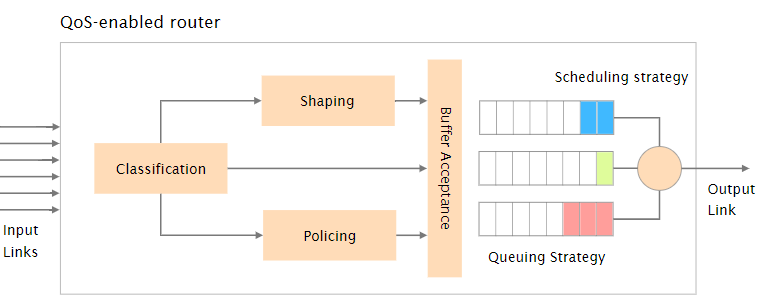
\includegraphics[scale=0.7]{images/2-qos.PNG}
	\caption{Components of a QoS enabled router.}
	\label{fig:qos}
\end{figure}

\subsection{Scheduling / Queuing Strategy}

%TODO more algos?

\paragraph{Scheduling}
Which buffered packets get send out next and when? Either work-conserving (link is never idle) or non-work conserving. Also, algorithms that maintain per-flow state typically do not scale. In practice, policies are combined to accommodate a number of classes of traffic.

\paragraph{FIFO} The first packet that arrives is the first one that leaves. Simple and no starvation but does not allow for prioritization and can be unfair.

\paragraph{Priority Queue}
Higher priority queues always get serviced first. Packets are classified. For each queue, packets serviced in a FIFO manner. Simple, allows for differentiation and isolating high priority traffic but starvation is a risk.

\paragraph{(Weighted) Fair Queue}
One queue per flow, round-robin to service all queues. Divide bandwidth among all flows equally. Weighted (fraction) allows for bandwidth allocation to each flow (not equal). Provides isolation and fairness (approximates max-min fair allocation, perfect if all packets have equal size - if not, smaller packets get penalized), but is very demanding resource-wise (one queue per flow) and thus doesn't scale. Perfect would be bit-by-bit queuing but way too complex and impossible. 

WFQ = FQ if weight for each queue is 1 over number of flows.
%TODO bit-by-bit approximation thingy

\paragraph{Max-Min Fairness}
Given a set of bandwidth demands $b_i$ and a total bandwidth $C$, the max-min bandwidth allocations $a_i$ are:

$$a_i = \text{min}(f, b_i)$$

where $f$ is the unique value (fair share) s.t. $\Sigma a_i = C$. This means that if a flow doesn't get full demand, no other flow gets more than the flow. Intuition: water filling different-capacity pipes, continue filling until no more water or all pipes full.

\begin{figure}[h]
	\centering
	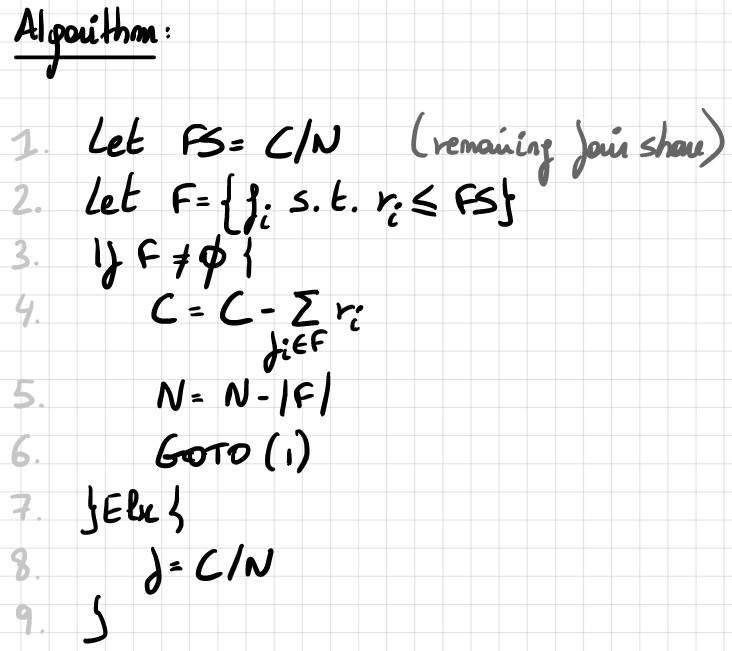
\includegraphics[scale=0.5]{images/2-maxmin.PNG}
	\caption{Computing Max-Min Fairness.}
	\label{fig:maxmin}
\end{figure}

%TODO algo example

\subsection{Buffer Acceptance}

After knowing which queue to append a packet to, router needs to decide whether to accept or drop it. By dropping packets, we signal to the sender to lower its rate (congestion).

\paragraph{Tail Drop}
Simply drop any newly arriving packets when the queue is full. Con: synchronizes TCP flows when multiple packets are lost (all sources backtrack the same). Also, it's completely agnostic.

\paragraph{Random Early Detection (RED)}
Instead of dropping when full, start dropping early as a preventive measure. The fuller the buffer, the more likely a packet is dropped. You're more likely to be dropped if you're causing the congestion. Randomness avoids global synchronization.

\begin{figure}[h]
	\centering
	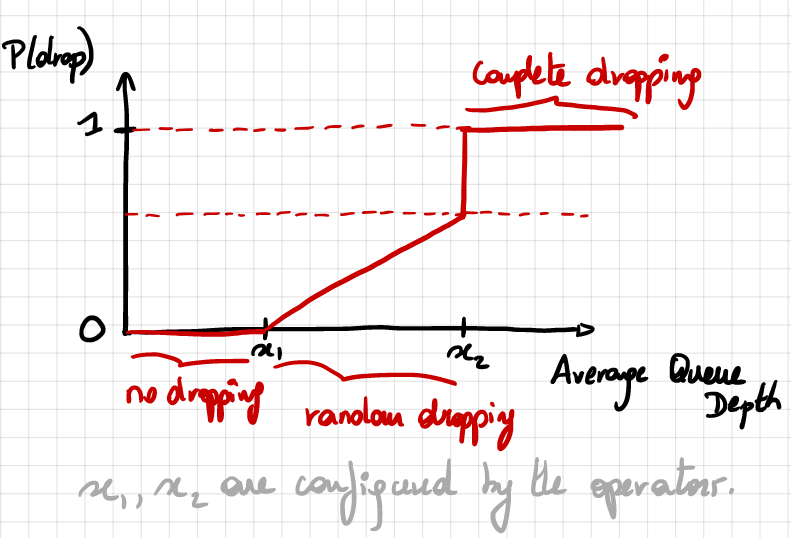
\includegraphics[scale=0.5]{images/2-red.PNG}
	\caption{RED visualized.}
	\label{fig:red}
\end{figure}

\subsection{Shaping and Policing}

\paragraph{Shaping}
Regulating the traffic by changing the outgoing rate.

\paragraph{Policing}
Specifying rules such as "only use x Gbps" and drop everything going over it.

\paragraph{Specifying Rates}
How to unambiguously characterize / monitor the throughput requirement of an application? By specifying / monitoring the burstiness of traffic (average rate and burst size) we can deal with both the max. rate and not be wasteful (don't just look at max or average).

\paragraph{Token Bucket Algorithm}
Used to check that sending rate conforms to defined limits on bandwidth and burstiness or can also be used as a scheduling algorithm.

Bucket with a fixed capacity filled with tokens representing units / bytes at a fixed rate. Every packet is checked by inspecting the bucket to see if it contains sufficient tokens at that time. If so, appropriate number of tokens is removed and packet is sent.

Conforming flows can contain traffic with average rate equal to bucket filling rate and burstiness determined by depth of bucket.

\begin{figure}[h]
	\centering
	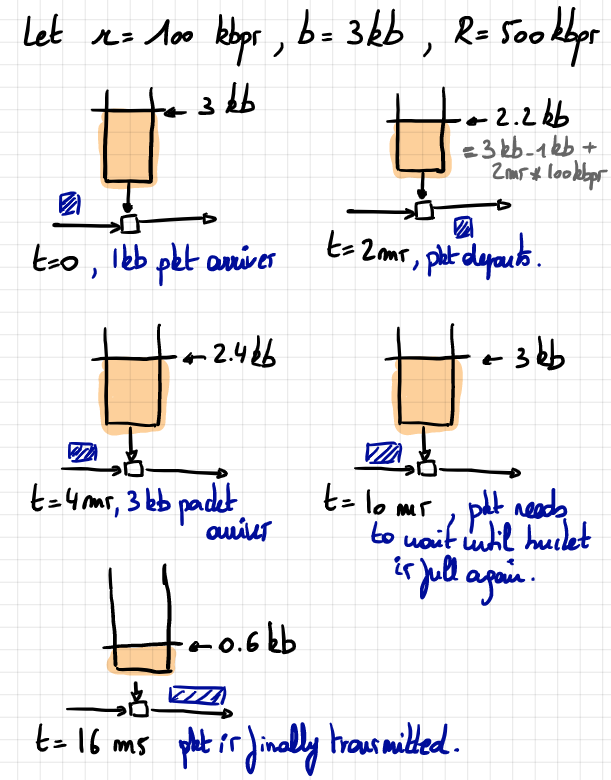
\includegraphics[scale=0.5]{images/2-bucketexample.PNG}
	\caption{Token Bucket example (filling rate, bucket depth and output rate).}
	\label{fig:bucket}
\end{figure}

\textbf{Non-Compliant Packets:} In the example, the non-compliant packet is delayed until it becomes compliant (shaping). One can also drop it (policing) or mark it (marking) which  gives the packet a lower priority. These are three things one can use a token bucket for.


%TODO lec 7 TB scheduling, classification what does it say

\subsection{Classification}

To enqueue packets in different queues with varying priorities, we need a way to classify them. For example, all TCP traffic is one class and all SSH traffic another. Or, customers are their own class. Anything can be a predicate to classify traffic and mark it accordingly.
\newpage

\section{Virtual Private Networks}

How to interconnect geographically distributed sites with the same privacy and guarantees as a private network on top of a shared infrastructure? High-level goals: support multiple customers, provide QoS guarantees, easy to use and manage for customer and provider.

\subsection{User-Managed VPN}

In a customer-managed VPN, provider is agnostic and simply provides dedicated physical connections (solution 1) or IP connectivity (solution 2).

\paragraph{Solution 1: Leased-Line}
A dedicated (private) full-duplex symmetrical connection between two geographically distant sites according to a commercial contract (e.g. provided by Swisscom). QoS guarantees easy since connection is dedicated and does not carry third-party communications. Either organized as a full mesh connecting all sites pairwise (redundancy) or as a hub-and-spoke where all sites are reachable but not specifically direct neighbors (cheaper).

Quality of connections is typically very good but it can be very expensive since you need many LLs (at least one per site). With $n$ sites and for a full mesh, one needs $\frac{n(n-1)}{2}$ LLs and $n$ interfaces on each router. Also, LL-based VPNs are not flexible since adding an LL can take months and adding / removing a site is a logistic nightmare.

\paragraph{Solution 2: IP-Based}
On each site, customer contracts simple IP connectivity with one or more providers (different IP subnets!). The customer then creates IP tunnels between its sites. The provider only needs to know the public IP addresses (11.0.0.0/8 in the example).

\textbf{IP Tunnel:} forwarding traffic across network that wouldn't normally support it (no existing native routing path to each other. Encapsulate traffic s.t. it carries a different header (= native) which the carrier network can process. There exist other tunneling protocols, plus IPsec also encrypts the original packet.

\begin{figure}[h]
	\centering
	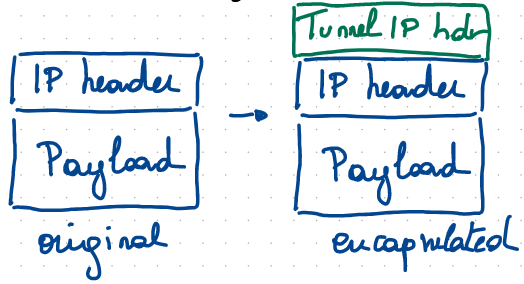
\includegraphics[scale=0.5]{images/3-tunnel.PNG}
	\caption{Additional IP header for tunneling (IP in IP) with source and destination addresses of the gateway routers.}
	\label{fig:tunnel}
\end{figure}

\begin{figure}[h]
	\centering
	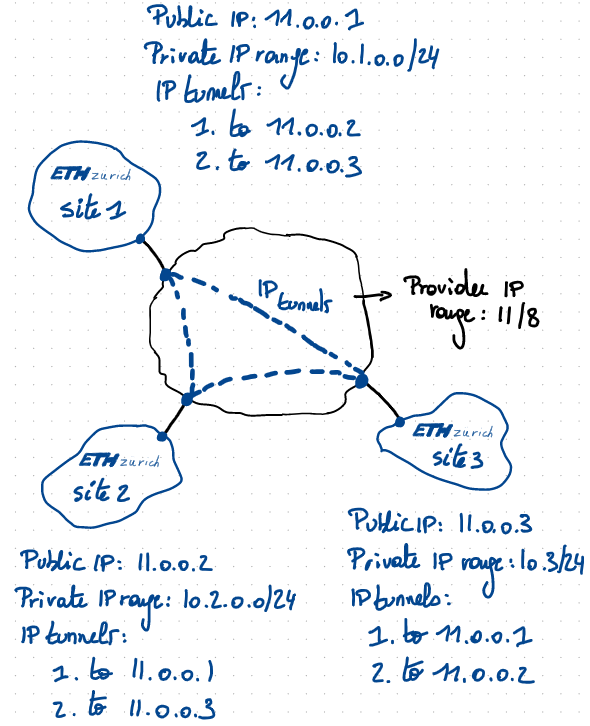
\includegraphics[scale=0.7]{images/3-ipexample.PNG}
	\caption{IP-based VPN infrastructure. Gateway routers native to transit network determine the tunnel to use and encapsulate outgoing packets accordingly.}
	\label{fig:ipexample}
\end{figure}

\textbf{Generic Routing Encapsulation (GRE):} can encapsulate many different protocols inside virtual point-to-point / to-multipoint links over IP (encapsulated packet has both an IP and a GRE header). GRE enables to give an insight into which protocol is encapsulated. See Figure \ref{fig:gre}.

\begin{figure}[h]
	\centering
	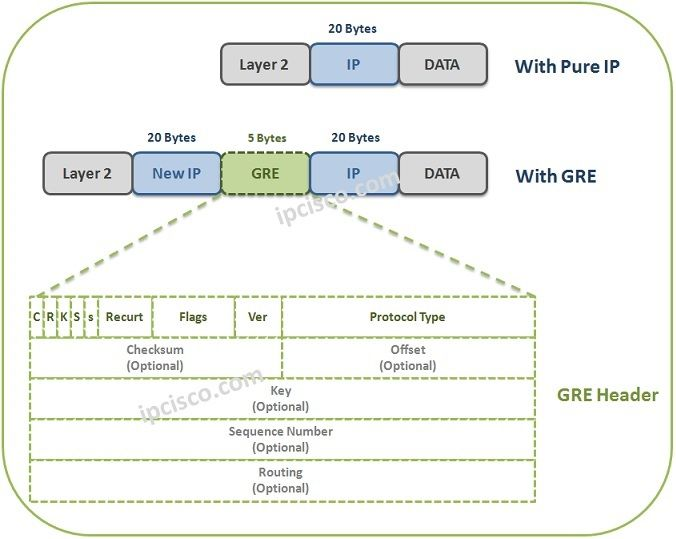
\includegraphics[scale=0.5]{images/3-gre.jpg}
	\caption{GRE header specification (note: Protocol Type indicating encapsulated protocol = EtherType).}
	\label{fig:gre}
\end{figure}

\textbf{Pros and Cons:} Much cheaper since each router (in each site) only requires one interface to connect to all others (or two for redundancy) since traffic is multiplexed. Again, total number of tunnels can be high (see full mesh connections). Adding a new site requires router config modification at all sites (if full mesh). Few guarantees are provided since provider is unaware that it is dealing with VPN traffic - only best-effort. VPN security depends on tunneling mechanism (weak for GRE, good for IPsec).


\subsection{Provider-Managed VPN}

The customer is agnostic to the service and it looks like the different sites are directly connected together through the provider. See Figure \ref{fig:provider} for an example architecture.

\begin{figure}[h]
	\centering
	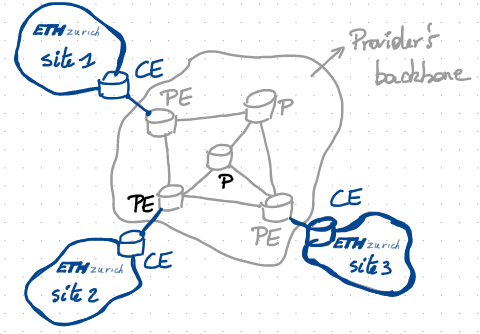
\includegraphics[scale=0.7]{images/3-provider.PNG}
	\caption{Architecture of a provider-managed VPN with CE, PE and P routers.}
	\label{fig:provider}
\end{figure}

\paragraph{Customer Edge (CE)}
Router sending IP packets through ISP backbone to reach other sites of the VPN. Always connected to a PE and does not now any details of ISP backbone.

CE routers only need one routing table containing routers of their own VPN (e.g. reach own site via local routing, reach different site via specific PE).

\paragraph{Provider Edge (PE)}
Maintains per-VPN config and ensures that packets sent by a site are delivered to PE attached to destination site.

In addition to the default routing table (backbone routes) they also maintain a dedicated routing table for each VPN a PE router is attached to - known as a VPN Routing and Forwarding table (VRF). Two packets from different VPNs with the same destination can map to different routes (next-hops) in their respective VRF on a PE router. See Figure \ref{fig:vrf} for an example.

\begin{figure}[h]
	\centering
	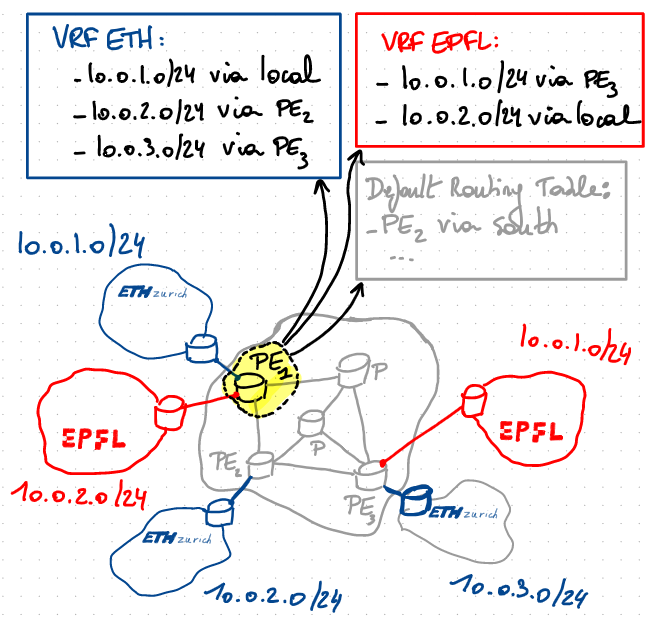
\includegraphics[scale=0.6]{images/3-vrf.PNG}
	\caption{Examples of VRFs for two VPNs.}
	\label{fig:vrf}
\end{figure}

%TODO: how are these packets marked / distinguished?

\paragraph{Provider (P)}
Routers withing ISP backbone. Unaware of VPN service.

P routers only need one routing table containing the routes of the backbone (how to reach P and PE routers).

%TODO hands-on example lec 8

\subsubsection{Routing}

%TODO difficult, check again, draw this? lec 8, print notes, examples

\paragraph{Distributing Routing Information}
First, each CE must advertise its local routes to its connected PEs. PEs in turn advertise the remote VPN routes to the CE (via static routes / configuration, eBGP, RiP, etc.).

Then, each PE must receive per-VPN routes reachable through local CE routers / remote PE routers and internal ISP routes to reach other PE routers (infrastructure routes, often going through a P router - plain OSPF).

Lastly, PE routers only advertise / receive internal routes. They don't know anything about VPN routes.

\begin{figure}[h]
	\centering
	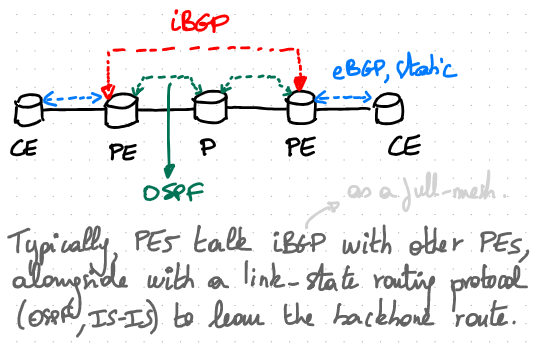
\includegraphics[scale=0.6]{images/3-routing.PNG}
	\caption{First and second step of distributing routing information.}
	\label{fig:routing}
\end{figure}

\paragraph{Dealing With Conflicting Info}
Different VPNs can use the same internal address space (e.g. ETHZ and EPFL both use 10.0.0.0/8) - same destination IP can map to different sites belonging to different VPN. Also, we want the CEs to only learn routes pertaining to their own VPN.

Concatenate a unique value to the IP address corresponding to the addressed VPN (8-byte Route Distinguisher, RD = 96-bit total address) and exchange that with Multiprotocol-BGP (MP-BGP) to solve the first problem.

Restrict the distribution of VPN-IPv4 routes using labels by assigning a unique label (= Route Target) to each VPN and have the PE router attach the tag to the BGP route before propagating it on iBGP. A PE router then only inspects routes associated with a given tag where they have a connected CE router.

Typically, both these labels are the same (RD and RT).


\subsubsection{Forwarding}

CE routers send pure IP packets, PE router encapsulates these with two MPLS labels (outer label identifying next-hop PE and inner label identifying VRF to use in remote PE).
\newpage

\section{Fast Convergence}

How to retrieve connectivity as fast as possible ($<$ 50 ms) after link / node failure?

\subsection{Overview}

\paragraph{Network / Routing Convergence}
A transition from a routing and forwarding state to another state typically triggered by a change in the topology (sudden in case of failure, planned / controlled in case of maintenance like hardware / firmware updates or config changes).

Convergence is a distributed process during which routers might have an inconsistent view of the network - this can lead to traffic loss or unnecessary depletion of resources (forward traffic to a blackhole or into a forwarding loop).

\paragraph{Sources of Delay}
Four steps: local detection of a failure, communication of the failure, recomputation and update of the forwarding state. First three steps are in the order of milliseconds. Last step in the order of number of prefixes that need to be updated which can be very slow (hundreds of seconds).


\subsection{IP Networks}


\subsubsection{Fast Detection}

Fast node / link failure detection with high accuracy and low overhead.

\paragraph{Physical- / Link-Layer Signals}
Some physical- / link-layers, such as optical layers, can detect failures through the loss of light or carrier signal (e.g. Synchronous Optical Networking - SONET, Synchronous Digital Hierarchy - SDH, Dense Wavelength Division Multiplexing - DWDM).

This is often as fast as possible (few ms) and has virtually no overhead. Cons: only works for some types of physical- / link-layers (e.g. not available on Ethernet) and does not detect certain kinds of failure (e.g. link between a router and switch fails but for other router connected to switch it seems like connection is still up - even tho router communication is broken).

%TODO: check out examples


\paragraph{Hello / Keepalive / Beacons}
Adjacent routers regularly exchange Hello messages and signal a failure whenever $k$ of those are missed in a row. By default, each routing protocol comes with such a mechanism and allows to configure: frequency (interval) and dead interval. Works on any router platform and detects a wider range of failures (since it actually tests the forwarding path), but it's slow and a huge overhead.

\paragraph{Bidirectional Forwarding Detection (BFD)}
Protocol-agnostic hello-based service running directly in the hardware (instead of relying on the numerous protocol-based mechanisms causing overhead). Since it is hardware-based (software is also possible), we can send frequent hellos without stressing the CPU (small hello and dead interval - 50ms and 150ms). Configure other protocols to not run their hello mechanisms anymore.

Session(s) established between two systems via three-way handshake that are explicitly configured (no discovery).

Fast detection, low overhead and high coverage (tests actual paths) - especially when run in hardware. Unfortunately, not all routers can run BFD in hardware (modern ones are more likely to have it).

\paragraph{Conclusions}
Use link-layer mechanism when available, complement with hardware-based mechanism and fallback on protocol-based ones as last resort.


\subsubsection{Fast Propagation}

Flooding of failure detection should happen immediately and flooded packets are sent with absolute priority over rest of traffic. Note that often, only parts of the network need to be informed of a failure for convergence.


\subsubsection{Fast Computation}

\paragraph{Shortest-Path-Based Protocols}
Like OSPF, IS-IS, etc. Not a huge problem anymore since computing an entire shortest-path tree in a huge network only takes a few ms nowadays and incremental shortest-path computation can help scale this process further (but most vendors don't even bother since first thing is so fast and incremental introduces complexity and possible bugs).

\paragraph{BGP}
Difficult since computation is done per-prefix and BGP routers often don't even know alternate paths and need to search for one (since only one route per prefix is advertised). There exist BGP extensions that allow for the advertisement of multiple routes for a prefix even if its not a chosen one (internal routers now need to carry many more route in their routing tables). Common tradeoff between scalability and speed.


%TODO BGP convergence lookup, example lec 9


\subsubsection{Fast Updates}

Updating the Forwarding Information Base (FIB) is typically the key bottleneck to overcome in the convergence process. Total update time = number of prefixes times average update time per prefix.

\paragraph{Cheap Trick}
Prioritize FIB updates according to how much traffic each prefix sees.

\paragraph{Long Term Solution}
Reorganize the FIB data structure (data plane) s.t. it allows for fast incremental updates. Pre-compute backup state, pre-load in reorganized FIB, activate pre-loaded backup state upon detecting a failure. IGP (Dijkstra-based protocols) - LFA and BGP - PIC.

\paragraph{Loop-Free Alternates (LFA)}
Neighbor that can carry your traffic impacted by the failure without it bouncing back to you (LFA does not use you to reach destination that you want to reach but can't). N is LFA for S to D if dist(N,D) $<$ dist(S,D) $+$ dist(S,N) (assumes symmetrical weights).

Depending on topology, a subset of the links / prefixes will be protectable by LFAs (e.g. triangles / meshes lead to high coverage vs. ring-based which suck). Coverage(per-link LFA) $\leq$ coverage(per-prefix LFA).

%TODO how to calculate LFA coverage?

\begin{figure}[h]
	\centering
	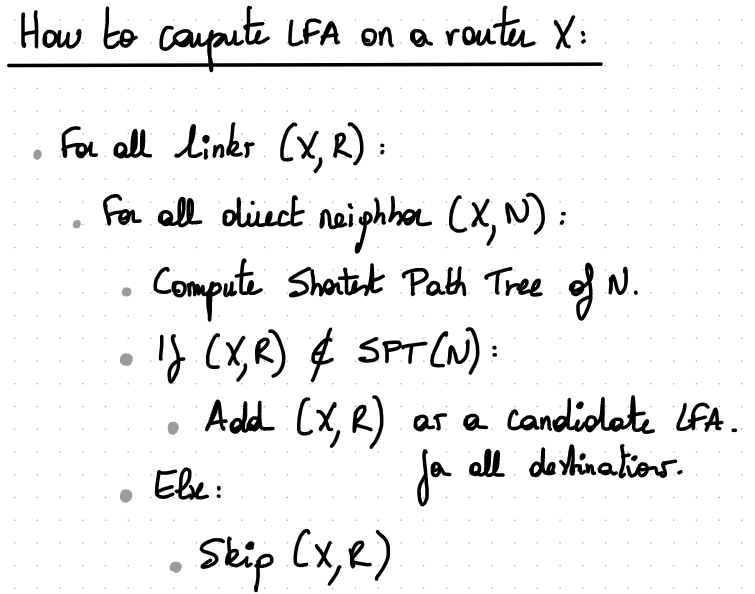
\includegraphics[scale=0.5]{images/4-lfa.PNG}
	\caption{Computing per-link LFAs for router X. Per-prefix LFAs can be calculated by evaluating each destination prefix instead each direct neighbor.}
	\label{fig:routing}
\end{figure}

%TODO examples lec 9

\textbf{Remote LFAs to increase coverage:} LFAs can be routers that are not directly connected by using tunneling (typically LDP-based). Does not guarantee full coverage!

\begin{figure}[h]
	\centering
	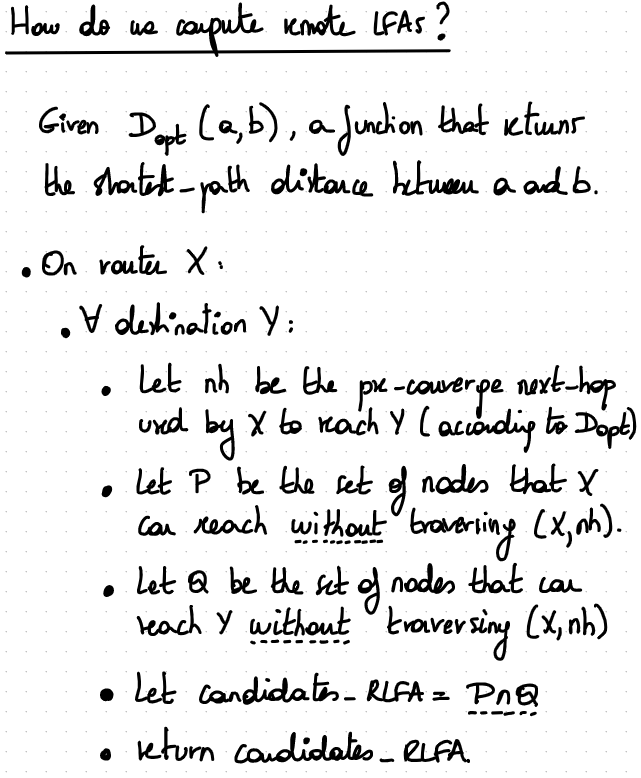
\includegraphics[scale=0.5]{images/4-remote.PNG}
	\caption{Computing remote LFAs.}
	\label{fig:remote}
\end{figure}

\textbf{FIB organization for fast activation:} one possible solution (which works well in P4) is to store two tables, one for mapping prefixes to a primary and a backup next-hop which are stored in the metadata of a packet and one for mapping each next-hop to a status (0 or 1) where if it's down (= 0) packet should use the backup next-hop.


\paragraph{Prefix-Independent Convergence (PIC)}
Enable the routers to quickly switch over to pre-installed alternate paths upon failures that affect BGP routes. The problem with standard BGP is "flat" FIBs where all reachable prefixes are mapped to a gateway routers egress interface.
%TODO ?????? google this


\subsection{MPLS Networks}

Easier than IP-based since we don't have distributed computations (as much).

Pre-establish secondary LSPs that don't carry any traffic to prepare for failures of important primary LSPs. Switching to the secondary LSP upon failure can be done immediately since there is no need for any coordination (provided the secondary LSP exists and is not impacted by the failure).

\subsubsection{End-To-End LSP Protection}

Ingress LSR establishes secondary LSP between ingress and egress LSR that relies on disjoint physical resources (router-disjoint and / or link-disjoint LSP) by using its path selection algo (signaled with RSVP-TE). Upon failure on primary LSP, adjacent router sends \textit{PathErr} message to ingress which triggers the switch to the secondary LSP.

Pro: ingress can immediately activiate secondary LSP without any coordination. Cons: one protection LSP must be established for each primary LSP, doubling the amount of memory needed. Failure info (\textit{PathErr}) must travel all the way to the ingress LSR before connectivity can be retrieved (slow!).


\subsubsection{Local LSP Protection}

Each LSR crossed by the primary LSP signals a protection LSP to cover for the failure of each link used by the primary LSP (can be generalized to router failures).

Pro: traffic can be immediately switches onto protection LSP by router detecting the failure (and not just by ingress). Con: depending on the network, a large number of protection LSPs might be required.

\begin{figure}[h]
	\centering
	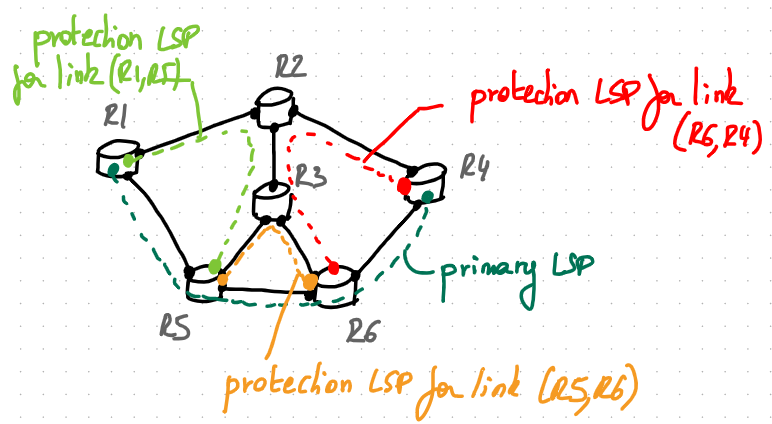
\includegraphics[scale=0.5]{images/4-local.PNG}
	\caption{Example for local LSP protection.}
	\label{fig:local}
\end{figure}
\newpage

\section{Multicast}

How to efficiently transmit data to a set of receivers. One or many to many.

\paragraph{Source-Based}
Sender simply sends as many copies of each IP packet as there are receivers (replication). Easy to implement but wastes a lot of bandwidth and is therefore not efficient.

\paragraph{Network-Based}
Sender transmit one copy of each IP packet like in IP unicast and network (i.e. the routers) take care of distributing this information to all the receivers (distribution tree). Efficient since each packet crosses each link only once but hard to implement (needs new protocols and forwarding mechanisms). Group of receivers is identified by a group address (multicast IP address).

\subsection{IP Multicast}

%TODO IPTV, IGMP and PIM, MOSPF

\paragraph{Addressing A Group Of Receivers}
A subset of the IP address space is reserved for multicast, namely 224.0.0.0 - 239.255.255.255 (leading bits are 1110) with some having pre-defined allocations (all hosts, all OSPF routers, etc.). Some of these can only be used within an AS (no public routing), namely 239.0.0.0 - 239.255.255.255.

\paragraph{Receiving Multicast Traffic}
On top of the physical MAC (L2) address (start with 0 in first byte), we can tell a host to listen to additional ones (logical addresses that identify a group of Ethernet destinations and start with 1 in first byte).

\paragraph{Multicast Address to MAC Mapping}
Take the 32-bit IPv4 multicast address and trim away the first 8 bits. The remaining 23 bits are the last 23 bits of the corresponding MAC address that always start with the same 25 bits (01:00:5e).

This process is not lossless, meaning that 32 IP multicast addresses are always mapped to the same logical Ethernet address. This can lead to unwanted traffic. Host needs to check the IP address and discard unwanted packets.

\paragraph{Router: Which Host is in Which Group?}
The Internet Group Management Protocol (IGMP) is used by hosts and adjacent routers (first-hop) to create multicast group membership. Hosts (repeatedly) tell / request from routers that they want the traffic with a specific IP destination address and routers keep track of that. Routers also periodically send out subscription queries. Adjacent routers use Protocol Independent Multicast (PIM) to direct traffic from hosts sending multicast traffic to hosts that requested it.

\paragraph{Dynamic Construction of Distribution Trees}
How do routers learn where the various receivers are and keep track of those over time (and where are the sources)?

\textbf{Pro-Active:} Hosts use IGMP to establish subscriptions and tell their first-hop routers and then a routing protocol is used to distribute group memberships s.t. each router knows the exact location of each group member (e.g. extend a link-state protocol as in MOSPF). Each router computes the shortest path tree (S, G) for each source S (original senders of multicast traffic) and group G (on demand whenever router receives a packet for G). Routers have full knowledge but memory overhead for all routers, flooding competes with normal link-state messages and as the number of sources and groups grows, computing the SPT can become problematic.

\textbf{Reactive:} Routers assume that receivers are everywhere and will initially broadcast the traffic (along shortest path tree with source as root) - only flood traffic when it arrives from SP upstream (Reverse Path Filtering - RPF). Unwanted branches are pruned by receiving stop requests from downstream routers that are not interested (or edge routers indicating that they have no hosts interested in traffic). This is called Flood-and-Prune. Approach is simple (plug and play) but costly since routers need to maintain per (S, G) state and flooding is frequently reactivated. There is also the hybrid mode that uses rendez-vous points: one router is the root of a shared distribution tree per group (configured in advance) and all routers know the address  - sources then encapsulate traffic to root and it multicasts the decapsulated traffic alongside shared traffic. Receivers dynamically join the shared tree.

\begin{figure}[h]
	\centering
	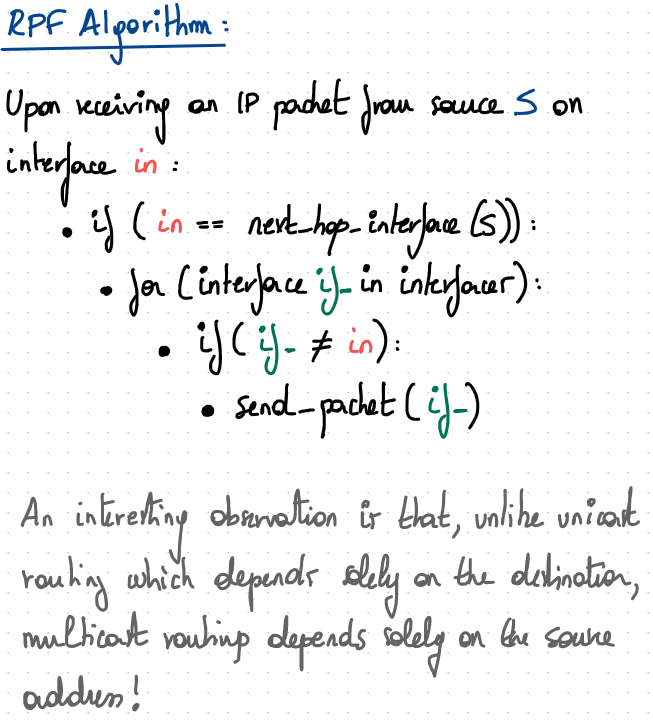
\includegraphics[scale=0.6]{images/5-rpf.PNG}
	\caption{Algo for Reverse Path Filtering.}
	\label{fig:rpf}
\end{figure}

\textbf{Avoiding Unnecessary Transmissions:} Sender-based solutions include each router computing the list of interfaces for each possible source on which to broadcast to s.t. it only includes interfaces on the SPT from a source (routers can rely on learned network topology). Receiver-based solutions include each router learning the list of outgoing interfaces on which to broadcast from for each source by having downstream routers tell them that a given interface is not on the shortest path (less intensive than sender-based) - router just broadcasts and downstream sends stop messages (as described in the Flood-and-Prune method).

%TODO ??

\textbf{Protocol Independent Multicast:} Most widely deployed multicast routing protocol. It leverages the existing unicast routing table to perform receiver-based optimization for RPF. Two modes: dense (Flood-and-Prune) or sparse (Rendez-Vous Points).

%TODO look this up

\newpage

\section{P4}

%TODO redefine code listing package thingy

%TODO expand with exercise knowledge / what have we seen

For this summary, the focus is on P4$_{16}$ and the \href{https://p4.org/p4-spec/docs/P4-16-v1.2.1.html}{P4 language specification version 1.2.1}. All concepts seen here are taken from the lecture and exercises only - of course, there is much more to the language, refer to the documentation for more. The following is a list of very helpful resources to get to know the P4 programming language:

\begin{itemize}
    \item \href{https://p4.org/p4-spec/docs/P4-16-v1.2.1.html}{P4 language specification version 1.2.1}
    \item \href{https://github.com/p4lang/p4c/blob/master/p4include/v1model.p4}{P4-16 declaration of the v1.0 switch model}
    \item \href{https://github.com/nsg-ethz/p4-learning}{P4 learning repository}
    \item \href{https://gitlab.ethz.ch/nsg/public/adv-net-2020/-/tree/master/}{All exercises of the lecture (including some non-P4 stuff like FRR)}
\end{itemize}

%TODO more

\subsection{Basics}

%TODO example program

\paragraph{Program Structure}
A P4 program consists of imported libraries (by using the \texttt{\#include <name.p4>} command), constant / variable declarations, a parser, the control flow (match-action pipeline), a deparser and a call to main.

To maintain state between packets, use tables or externs (register, etc.).

The only loop possible in P4 is when we need to parse a header stack.

The most basic function of a switch (L2) is to compute the next hop, update the MAC addresses, decrease the TTL and forward it to the right egress port.

\paragraph{Base Types}
P4 is statically-typed and includes base types, as well as operators to derive composed ones (see below). Base types include (there is no float or string):

\begin{itemize}
    \item \texttt{bool}, default false
    \item \texttt{bit<n>}, width n, default 0
    \item \texttt{int<n>}, signed int, width n, default 0
    \item \texttt{varbit<n>}, dynamic length $\leq$ n
    \item etc.
\end{itemize}


\paragraph{Constant and Variable Declarations}
Declare constants and variables with these constructs (examples): 

\begin{itemize}
    \item \texttt{const bit<16> TYPE\_IPV4 = 0x800;}
    \item \texttt{typedef bit<32> ip4Addr\_t;}
    \item \texttt{header ip4\_t \{...\}}
    \item \texttt{struct headers \{...\}} or \texttt{struct metadata \{...\}} - unordered collection of named members
    \item \texttt{tuple<bit<32>, bool> x;} with \texttt{x = \{10, false\};} - unordered collection of unnamed members
\end{itemize}


%TODO tuples

\paragraph{Operations}
P4 includes arithmetic operations (add, sub, mult) without division and modulo, bitwise operators (complement, and, or, bit shift, xor), relation operators (smaller, bigger, equal, etc.), bit-slicing / concatenation, etc. 

\paragraph{Header Type}
The \texttt{header} type is similar to a \texttt{struct} in C and contains all the fields of the header to be defined at the beginning of the program. A header cannot be nested and contains a hidden Boolean validity field - the header is valid if this bit is true (use \texttt{isValid(), setValid(), setInvalid()} to manipulate it). A successful \texttt{extract()} during the parsing stage sets the validity bit to true. Example:

\begin{lstlisting}
header Ethernet_h {
   bit<48> dstAddr;
   bit<48> srcAddr;
   bit<16> etherType;
}
\end{lstlisting}

To declare a header, use \texttt{Ethernet\_h ethernetHeader;} or \texttt{MPLS\_h[10] mpls;} for a header stack with size 10. Headers are often combined by declaring them in a \texttt{struct} with the name \texttt{headers}. One can also define a \texttt{header\_union} where only one included alternative can be present (e.g. IPv4 vs. IPv6).

\paragraph{Metadata}
Intermediate data generated and / or manipulated during the execution of a P4 program and only associated with a single packet (if not used in combination of some kind of memory like registers). Can either be user-defined or is intrinsic to the underlying architecture model used (\texttt{struct standard\_metadata\_t}) - e.g. the ingress port of the packet or timestamps. %TODO: more? 

For this lecture, the architecture used is the \textit{v1model.p4}.

\paragraph{Externs}
Blackbox functions with a known interface and intrinsic to the architecture model used (kinda like Java interfaces). Can also be described as stateful objects. The \textit{v1model.p4} includes registers that store arbitrary data, counters, meters that can limit the rate, etc.

\begin{figure}[h]
	\centering
	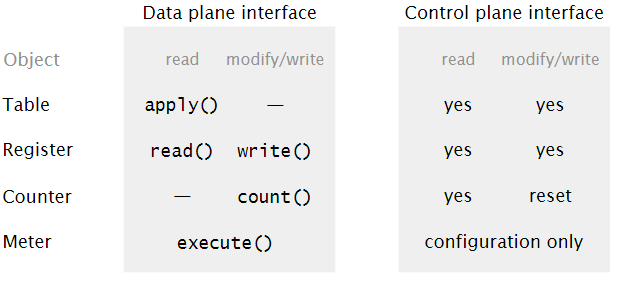
\includegraphics[scale=0.6]{images/6-externs.PNG}
	\caption{Stateful objects in P4 / v1model.}
	\label{fig:externs}
\end{figure}

%TODO: more on reg, counter, meter

\paragraph{Directional Parameters}
A function can take \texttt{in} parameters (only read inside the function), \texttt{out} parameters (uninitialized and written inside function, return values) and \texttt{inout} parameters (kinda like call-by-reference). Action parameters resulting from a table lookup (see below) don't have a direction since they come from the control plane.

\subsubsection{Parser}

%TODO what happens if reject - just dropped?
%TODO: in, out, inout things, function inputs

The parser maps packets into headers and metadata used and manipulated during the control flow stage of the P4 processing pipeline. It always needs to have a \texttt{start} state. In every state, one can transition into another state, which may depend on some condition, or transition into the \texttt{accept} resp. \texttt{reject} state (which is the default if no transition is specified). 

There are more advanced concepts that can be used in a parser (error handling with verify, accessing bits that are not parsed yet with lookahead, subroutines with sub-parser) - not really used during lecture / exercises. %TODO right?

Example of a common parser, with which we can later use \texttt{hdr}, \texttt{meta} and \texttt{standard\_metadata} of an IPv4 TCP resp. UDP packet:

\begin{lstlisting}
parser MyParser(packet_in packet,
                out headers hdr,
                inout metadata meta,
                inout standard_metadata_t standard_metadata) {

    state start{
        transition parse_ethernet;
    }
    
    state parse_ethernet{
        packet.extract(hdr.ethernet);
        transition select(hdr.ethernet.etherType){
            0x800: parse_ipv4;
            default: accept:
        }
    }
    
    state parse_ipv4{
        packet.extract(hdr.ipv4);
        transition select(hdr.ipv4.protocol){
            6: parse_tcp;
            17: parse_udp;
            default: accept;
        }
    }
    
    {...}
}

\end{lstlisting}


\subsubsection{Match-Action Pipeline}

After parsing the incoming packet, its checksum can be verified, ingress and egress processing is applied and its checksum can be updated - all using the information extracted during the parsing stage. All of these stages are divided into their own control blocks which are kinda like methods. Each block can contain its own variable and constant declarations and will most likely contain action and table declarations (= match-action units) and an (empty) apply statement defining the control flow.

\paragraph{Packet Checksum}
hmm, ip thingy %TODO

\paragraph{Ingress vs. Egress Processing}
I have no idea what the difference is. For the purpose of this lecture and the exercises, we almost always only defined any code in the ingress stage. %TODO

\paragraph{Processing Control}
An ingress / egress control block almost always contains constant / variable declarations, actions, tables and an apply statement. More advanced concepts include packet cloning, sending packets to the control plane and recirculating a packet.

\paragraph{Action}
Defines a function called when matching a specific key in a table. Can have zero or many input values extracted during the parsing stage.


\begin{lstlisting}
action drop() {
    mark_to_drop(standard_metadata);
}

action ipv4_forward(macAddr_t dstAddr, egressSpec_t port) {
    hdr.ethernet.srcAddr = hdr.ethernet.dstAddr;
    hdr.ethernet.dstAddr = dstAddr;
    standard_metadata.egress_spec = port;
    hdr.ipv4.ttl = hdr.ipv4.ttl - 1;
}
\end{lstlisting}

\paragraph{Table}
The control plane of a switch keeps track of all the tables used to process a passing packet. A table maps one or multiple given keys (header or metadata values extracted from the packet or else) to one of possibly many defined actions. The actual content of a table is filled by and stored in the control plane, while the structure of it is defined in the P4 program.

%TODO: how to fill

\begin{lstlisting}
table mpls_tbl {
    key = {
        hdr.mpls.label: exact;
    }
    actions = {
        mpls_forward;
        drop; // could also be NoAction
    }
    default_action = drop;
    size = CONST_MAX_LABELS;
}
\end{lstlisting}

\paragraph{Match Types}
A key can be matched either one-to-one (\texttt{exact}), longest prefix match (\texttt{lpm}) and ternary which TODO . The \textit{v1model.p4} also includes range match (check if a value is between x and y).

%TODO more detail, ternary

\paragraph{Filling a Table}
The .json topology object that describes all nodes and connections of a network also includes the possibility to define a .txt input file that defines CLI commands for a specific switch. To fill a table of a switch, the .txt file includes lines like:

\texttt{table\_add table\_name action\_name key $=>$ input\_1 ... input\_n}

\paragraph{Apply Statement}
Defines when to apply which table (and more). Can use if-else, switch, etc. statements. Example:

%TODO: more, switch example

\begin{lstlisting}
apply {
    table_1.apply();
    
    // Is it an IPv4 packet?
    if(hdr.ipv4.isValid()){
        table_2.apply();
    }
    
    // Apply table and check if there is a hit
    if(table_3.apply().hit){...}
    
    // Apply table and check which action is executed
    switch(table_4.apply().action_run){
        action1: {...}
        action2: {...}
    }
    
    {...}
}
\end{lstlisting}




\subsubsection{Deparser}
Puts packet back together s.t. it can be processed by regular switches in the network. Example: %order? if else stuff

\begin{lstlisting}
control MyDeparser(packet_out packet, in headers hdr) {
    apply {
        packet.emit(hdr.ethernet);
        packet.emit(hdr.mpls);
        packet.emit(hdr.ipv4);
    }
}
\end{lstlisting}
\newpage

\section{FRRouting}
\newpage

\section{Exercises}

%TODO: include examples?

\subsection{Tutorials}

\subsubsection{Reflector and Repeater}

The reflector sends the packet back to where it came from (swap MAC and set egress port to ingress port) and the repeater sends a packet to the port where the packet did not arrive on (match exact on ingress port, forward based on matched table entry - P1 to P2 and vice versa).

Solution omitted.

\subsubsection{L2 Fun}

First, we do simple L2 forwarding where we match the destination MAC address to a specified egress port.

Then, we do L2 broadcasting. If the destination MAC address is \texttt{FF:FF:FF:FF:FF:FF}, a switch sends a packet to all the ports the packet did not come from. For this multicast to work, the packet needs to be replicated and send to a multicast group. With four ports, we need four different multicast groups so that we don't send the packet back to the ingress port when broadcasting. First, define four multicast nodes with their replication ID (first number) as follows (CLI):

\begin{lstlisting}
mc_node_create 0 2 3 4
mc_node_create 1 1 3 4
mc_node_create 2 1 2 4
mc_node_create 3 1 2 3
\end{lstlisting}

Then, associate each multicast node with a multicast group:

\begin{lstlisting}
mc_mgrp_create 1
mc_node_associate 1 0

mc_mgrp_create 2
mc_node_associate 2 1

mc_mgrp_create 3
mc_node_associate 3 2

mc_mgrp_create 4
mc_node_associate 4 3
\end{lstlisting}

In the P4 program, we define two tables: one to map a multicast group to an ingress port (e.g. ingress port 1 is mapped to group 1 since it excludes port 1) in case of a broadcast (this automatically forwards the packet correctly with \texttt{standard\_metadata.mcast\_grp = mcast\_grp;}) and one to simply forward to the right port in case of unicast (match on destination MAC address).

In the third exercise, we %TODO: digest and copy exercise


\subsubsection{Basic Load Balancing}



\subsubsection{Probabilistic Data Structures}

\subsubsection{L3 Fun}

\subsubsection{Congestion Aware Load Balancing}

\subsubsection{Packet Loss Detection}



\subsection{MPLS}

\subsection{RSVP}

\subsection{Load Balancing}

\subsection{Traffic Control}

\subsection{MPLS VPN and VRF}

\subsection{Fast Reroute}

\subsection{IP Multicast}
\newpage

\end{document}